\chapter{Methodology} \label{sec:methodology}

As summarized by the survey paper \cite{nid_ml_survey_2019} of Hongyu Liu and Bo Lang in section \ref{section:stateofart:nid_machine_learning_survey}, the design space for \gls{ml} based \gls{nids} is vast and can be hard to navigate at times. Hence, careful consideration of data representation, data pre-processing, \gls{ml} models, model parameters and training hyperparameters is necessary. The goal of the thesis was to examine the benefit of pre-training for already established \gls{dl} models in the context of \gls{nids}, hence we wanted to start from the most effective \gls{dl} models available, which, derived from state-of-the-art research, seems to be a uni-directional multi-layer \gls{dlstm} network. Additionally, we also looked at research on \gls{dl} and self-supervised/unsupervised learning in general. Most of the state-of-the-art research on \gls{dl}, and especially in self-supervised/unsupervised and transfer learning, is done in the context of \gls{nlp} \cite{bert}, \cite{elmo}, \cite{attention}.

Network communication is similar to natural language in the sense that it follows a certain set of rules, a grammar so to say, and each token like a word or packet conveys some semantic meaning when in the context of a sentence or flow. Other researchers have made similar observations \cite{anomaly_detection_recurrent_neural_networks}. We deemed the TransformerEncoder, which is often cited as an advancement of the \gls{lstm} in sequence modeling, to be a powerful new tool for network traffic classification. 

\section{Datasets} \label{sec:methodology:datasets}

We used the two \gls{nids} datasets \textit{UNSW-NB15} \cite{unsw_nb15} and \textit{CIC-IDS-2017} \cite{cic_ids_2017}. \par

The \textbf{UNSW-NB15} dataset \cite{unsw_nb15}, created by Nour Moustafa et al. from the School of Engineering and Information Technology, University of New South Wales at the Australian Defence Force Academy, Australia, was released as an update for the formerly frequently used but deprecated \cite{unsw_nb15} KDD dataset family. It was designed to reflect most known low foot print attacks at time of publication. The records are bidrectional flows extracted from the raw traffic data and grouped by the commonly used \textit{<srcIP, dstIP, srcPort, dstPort, protocol>} tuple. Each flow is described by 47 derived or measured features e.g. total duration, bytes transmitted, the mean of the flow packet size transmitted by destination IP, etc. After preprocessing where some incomplete records are removed, the dataset contains a total of 2.06 million records of which 1.99 million are normal transactions labeled as benign and 0.072 million attack records meaning 96.64\% of data is classified as benign and 3.36\% as attack. Attack records can be further divided into nine attack categories as listed in table \ref{table:methodology:datasets:unsw_nb15_categories}.

\begin{table}[H]
	\centering
	\begin{tabular}{cccccc}
		\thead{\textbf{\#}} & \thead{\textbf{Class}} & \thead{\textbf{\textbf{No. Records}}} & \thead{\textbf{\% w.r.t.} \\ \textbf{benign class}} & \% \thead{\textbf{\% w.r.t.} \\ \textbf{majority atk. class}} & \thead{\textbf{\% w.r.t.} \\ \textbf{total instances}} \\ \hline \midrule
		0  & Analysis       & 534         & 0.03\%                 & 1.82\%                        & 0.03\%                    \\ \midrule
		1  & Backdoors      & 397         & 0.02\%                 & 1.36\%                        & 0.02\%                    \\ \midrule
		2  & DoS            & 3972        & 0.20\%                 & 13.57\%                       & 0.19\%                    \\ \midrule
		3  & Exploits       & 29281       & 1.47\%                 & 100.00\%                      & 1.42\%                    \\ \midrule
		4  & Fuzzers        & 20848       & 1.05\%                 & 71.20\%                       & 1.01\%                    \\ \midrule
		5  & Generic        & 4301        & 0.22\%                 & 14.69\%                       & 0.21\%                    \\ \midrule
		6  & Benign         & 1991349     & 100.00\%               & 6800.82\%                     & 96.46\%                   \\ \midrule
		7  & Reconnaissance & 11971       & 0.60\%                 & 40.88\%                       & 0.58\%                    \\ \midrule
		8  & Shellcode      & 1546        & 0.08\%                 & 5.28\%                        & 0.07\%                    \\ \midrule
		9  & Worms          & 185         & 0.01\%                 & 0.63\%                        & 0.01\%                   
	\end{tabular}
 	\caption{UNSW-NB15 dataset record distribution \cite{unsw_nb15}.}
 	\label{table:methodology:datasets:unsw_nb15_categories}
\end{table}

The dataset was generated from a synthetic environment comprised of 3 networks and 45 distinct IP addresses using the IXIA PerfectStorm (now keysight PerfectStorm) tool.

The \textbf{CIC-IDS-2017} dataset \cite{cic_ids_2017}, created by Iman Sharafaldin et. al from Canadian Institute for Cybersecurity (CIC), University of New Brunswick (UNB), Canada constitutes another updated representation of known attack types at the time of publication. Compared to the UNSW-NB15 dataset it contains records of more modern cyber attacks like Heartbleed, HULK DoS but leaves out e.g. worm attacks. It contains a total of 2.31 million records of which 1.73 million are labeled as benign and 0.58 million are attack records. In other words, 74.72\% of the dataset are benign records and 25.28\% attack records. Attack records are further classified as shown in table \ref{table:methodology:datasets:cic_ids_2017_categories}.

\begin{table}[H]
	\centering
	\begin{tabular}{cccccc}
		\thead{\textbf{\#}} & \thead{\textbf{Class}} & \thead{\textbf{No. Records}} & \thead{\textbf{\% w.r.t.} \\ \textbf{benign class}}s & \thead{\textbf{\% w.r.t.} \\ \textbf{majority atk. class}} & \thead{\textbf{\% w.r.t.} \\ \textbf{total instances}} \\ \hline \midrule
		0  & Botnet ARES             & 755         & 0.04\%                 & 0.32\%                          & 0.03\%                    \\ \midrule
		1  & FTP-Patator             & 254         & 0.01\%                 & 0.11\%                          & 0.01\%                    \\ \midrule
		2  & SSH-Patator             & 2556        & 0.15\%                 & 1.09\%                          & 0.11\%                    \\ \midrule
		3  & DDoS LOIT               & 94327       & 5.46\%                 & 40.39\%                         & 4.08\%                    \\ \midrule
		4  & DoS GoldenEye           & 7451        & 0.43\%                 & 3.19\%                          & 0.32\%                    \\ \midrule
		5  & DoS Hulk                & 233521      & 13.53\%                & 100.00\%                        & 10.11\%                   \\ \midrule
		6  & DoS Slowhttptest        & 4209        & 0.24\%                 & 1.80\%                          & 0.18\%                    \\ \midrule
		7  & DoS slowloris           & 3886        & 0.23\%                 & 1.66\%                          & 0.17\%                    \\ \midrule
		8  & Heartbleed              & 2           & 0.00\%                 & 0.00\%                          & 0.00\%                    \\ \midrule
		9  & Infiltration            & 76237       & 4.42\%                 & 32.65\%                         & 3.30\%                    \\ \midrule
		10 & Benign                  & 1726226     & 100.00\%               & 739.22\%                        & 74.72\%                   \\ \midrule
		11 & PortScan - Firewall off & 159648      & 9.25\%                 & 68.37\%                         & 6.91\%                    \\ \midrule
		12 & PortScan - Firewall on  & 381         & 0.02\%                 & 0.16\%                          & 0.02\%                    \\ \midrule
		13 & SQL Injection           & 13          & 0.00\%                 & 0.01\%                          & 0.00\%                    \\ \midrule
		14 & XSS WebAttack           & 678         & 0.04\%                 & 0.29\%                          & 0.03\%                   
	\end{tabular}
	\caption{CIC-IDS-2017 dataset record distribution \cite{cic_ids_2017_analysis}.}
	\label{table:methodology:datasets:cic_ids_2017_categories}
\end{table}

In contrast to the UNSW-NB15 network simulation environment, the network topology consists of two networks: A highly secured victim network with firewall, router, switches and most common operating systems. The attack network is a separate network, containing a set of PCs with public IPs and running Windows 8.1 and Kali Linux.

To reduce variance in results and to keep comparability high we use the same random seed for all experiments and use stratified sampling when we divide the data sets into smaller chunks for pretraining, training and validation to assure the each attack category is represented in the subset proportionally to the whole dataset. This is especially important if we use very small subsets (10 flows per attack category) for finetuning as described in section \ref{sec:experiments}. 

\section{Data Representation}

Network traffic data can be viewed from a multitude of perspectives ranging from aggregate statistical data over different time-frames \cite{kitsune} to looking at feature representations of single packets. These can be viewed in the context of \textit{flows}.
Flows are loosely defined as sequences of packets that share a certain property \cite{adversarial_recurrent_ids}. In our case we define flows as sequences of packets that share source and destination IP address, source and destination port, and the network protocol used. This creates the quintuple \textit{<srcIP, dstIP, srcPort, dstPort, protocol>} as the key over which individual packets are aggregated to flows, which is a very common approach \cite{caia_vector}, \cite{unsw_nb15}, \cite{feature_vectors}. We chose a flow representation since this approach has shown good results frequently, is easy to obtain, requires no domain knowledge, and is feasible for encrypted traffic \cite{feature_vectors}. The downside of this approach is that the packet payload is ignored, which leads to poor classification performance for \gls{u2r} and \gls{r2l} \cite{nsl_kdd} like SQL injection, XSS and other payload based attacks. This is also shown by our results as can be seen in section \ref{sec:results}.
Commonly, flows are represented as a single feature vector in the dataset, containing aggregated statistical data of the completed flow like e.g. the mean of the flow packet size transmitted by the source IP, source to destination packet count or bits per second or total duration of the transmission. The downside of this is that flows can be processed only once they are completed \cite{adversarial_recurrent_ids}. In a real world scenario, this approach has major downsides since the \gls{ids} can only inspect communications in retrospect and never in real time. This was one of the reasons we decided to represent our flows as a sequence of packets instead of a single aggregated feature vector. Each packet is represented by the 15 features in table \ref{table:methodology:data_representation:features}.

\begin{table}[H]
	\centering
	\begin{tabular}{c c c c l}
		\thead{\textbf{\#}} & \thead{\textbf{Name}} & \thead{\textbf{Type}} & \thead{\textbf{Constant} \\ \textbf{over flow}} & \thead{\textbf{Description}} \\ \hline \midrule
		0 & srcPort & Int & yes & Source port number \\ \midrule
		1 & dstPort & Int & yes & Destination port number \\ \midrule
		2 & protocol & Int & yes & Protocol identifier \\ \midrule
		3 & pktLength & Int & no & Destination port number \\ \midrule
		4 & pktIat & Int & no & \gls{iat} \\ \midrule
		5 & pktDirection & Bool & no & Sending direction of the packet \\ \midrule
		6 & synFlag & Bool & no & TCP SYN Flag \\ \midrule
		7 & finFlag & Bool & no & TCP FIN Flag \\ \midrule
		8 & rstPort & Bool & no & TCP RST Flag \\ \midrule
		9 & pshFlag & Bool & no & TCP PSH Flag \\ \midrule
		10 & ackFlag & Bool & no & TCP ACK Flag \\ \midrule
		11 & urgFlag & Bool & no & TCP URG Flag \\ \midrule
		12 & eceFlag & Bool & no & TCP ECE Flag \\ \midrule
		13 & cwrFlag & Bool & no & TCP CWR Flag \\ \midrule
		14 & nsFlag & Bool & no & TCP NS Flag \\ \midrule
	\end{tabular}
	\caption{Packet features \cite{cic_ids_2017_analysis}.}
	\label{table:methodology:data_representation:features}
\end{table}

Another reason why we used a packet sequence instead of an aggregate flow representation is its similarity to natural language as mentioned before, which enables us to apply state-of-the-art methods from \gls{dl} based \gls{nlp}. We used the data pre-processing from \cite{adversarial_recurrent_ids} as it fit the requirements for our experiments and was easily modifiable.

To keep gradient paths shorter and to improve training stability, packet sequences are truncated to be at most 100 packets long. As last step of pre-processing features are normalized to be within a range of $[-1,1]$ to make gradient descent converge quicker.

\begin{figure}[h]
	\centering
	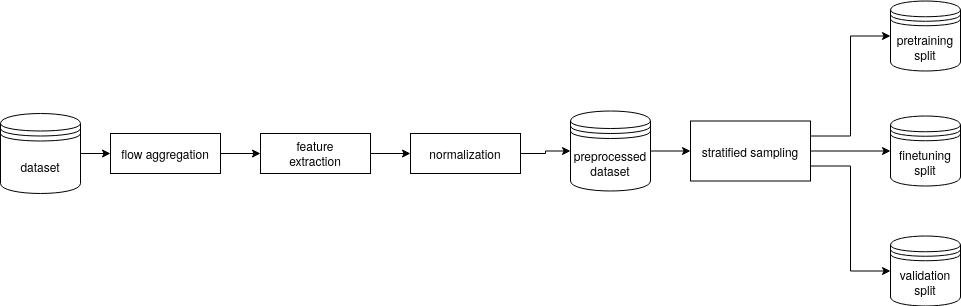
\includegraphics[width=0.95\linewidth]{graphics/img/dataset_preprocessing.png}
	\caption{All steps performed in dataset preprocessing to yield pretraining, training and validation splits.}
	\label{fig:dataset_preprocessing}
\end{figure}

\section{Machine Learning Models}

To inspect the potential benefits of self-supervised pretraining for \gls{ml}-based intrusion detection we chose to take a look at \gls{lstm} and Transformer networks as they are suited to process sequences of variable length and have shown promising results in the past in the domains of \gls{ids} and/or \gls{nlp} \todo{give examples}. Both types of networks are generally susceptible to improvements through self-supervised pretraining as prior research has shown \cite{bert} \cite{unsupervised_learning_lstms} \cite{unsupervised_learning_lstms_timeseries}. Whether pretraining improves performance in the context of \gls{nids} remains to be shown and is subject of this thesis.

For our \textbf{\gls{lstm} network} we chose a three layer \gls{dlstm} with a \textit{hidden size} of 512. While a larger network might be slightly more effective, this configuration proved to be swiftly trainable while also producing results close to those achieved by other researchers using \gls{lstm} models applied to the same datasets \cite{fog_based_detection_survey_2020}. Since our main focus is on comparisons between different training methods applied to the same model, it is not necessary to achieve optimal results as this would unnecessarily increase the training time needed until the model converges. For training the \gls{lstm} model, each flow is considered one sample and each packet is one token. The tokens are processed by the model in chronological order, meaning packets with an earlier timestamp will be processed first. The timestamp however is not part of the feature representation but is considered for data pre-processing to order packets within flows. Independent of the context, \gls{lstm} models have shown to be sensible to initialization of their weights and hidden state. This can be seen as a drawback but also as an opportunity to increase performance or decrease learning time. While there are many ways to initialize the parameters of an \gls{lstm} network, the most common ones are 0-initialization, random initialization and some form of transfer learning which in our case is self-supervised pretraining. For pretraining, the output layer is a linear layer with 15 nodes, equal to the number of features, and no activation function. For binary classification the output layer is replaced with a linear layer with a single node and no activation function because the objective function binary classification \gls{bce} loss operates on logits. This results in a sequence2sequence model which generates output sequences equal to the length of the input sequence. For pre-training this is the desired result, but for binary classification would only require a sequence2scalar model. So for classification, only the output of the last stage is looked at because at that point, the whole input sequence was processed by the model and information in a (uni-directional) \gls{lstm} only flows in one direction. The output of this stage should therefore be most accurate.

\begin{figure}[h]
	\centering
	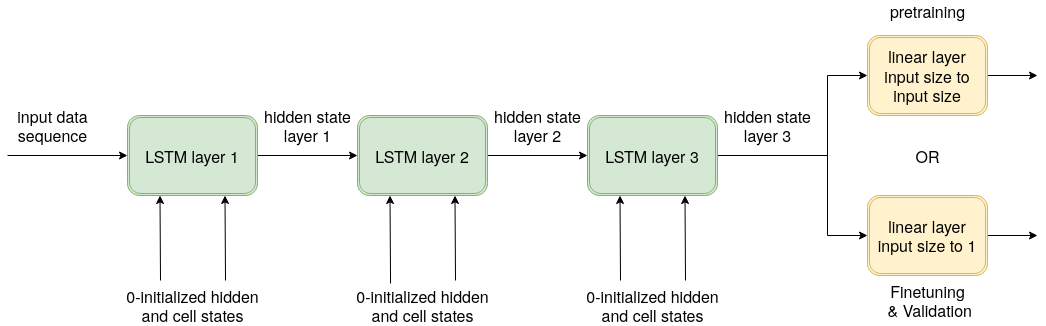
\includegraphics[width=0.95\linewidth]{graphics/img/lstm_model.png}
	\caption{Depiction of the \gls{lstm} model.}
	\label{fig:lstm_model}
\end{figure}

The Transformer model as proposed by Vaswani et. al \cite{attention} and its derivative score high on the leader boards of \gls{nlp} benchmarks like GLUE \cite{glue} or SQuAD \cite{bibid} and are still considered state-of-the-art in many regards. Following the example of \gls{bert} we only used the encoder part of the \textit{Transformer network} since the decoder does not provide any benefits for classification problems. We tuned the model parameters to be 10 Transformer layers, each layer consisting of a 3-headed Multi-Head Attention block and a feed-forward network with a forward expansion of 2, meaning an internal representation size double to the number of features per packet. For pretraining, the output layer is a linear layer with 15 nodes, equal to the number of features, and no activation function. For binary classification the output layer is replaced with a linear layer with a single node and no activation function because the objective function for binary classification \gls{bce} loss operates on logits. This again results in a sequence2sequence model which produces output sequences of length equal to the input sequence. For binary classification, we only need a single value, but the Transformer Encoder model produces a sequence of values. In contrast to the \gls{lstm} model, information in the Transformer does not aggregate at a specific stage and therefore we can't identify an output token which has more information or is more likely to be accurate than others. Google solved this problem for \gls{bert} by prepending a classification token to every input sequence and the model learns to aggregate information regarding classification at the corresponding output token. We tried this approach with no success, perhaps due to insufficient training. We opted for an average pooling layer over all output tokens to get from a sequence of variable length to a single value and this approach also works as can be seen later in the results section \ref{sec:results:transformer}.

\todo{insert image of transformer model}

\section{Framework and Training}

To conduct our experiments we used PyTorch \cite{pytorch} to implement and train our proposed models. To save labor and to keep results comparable we used the standard implementations \textit{torch.nn.LSTM} and \textit{torch.nn.TransformerEncoder}. Training is conducted by a standard training loop going through forward and back propagation, calculating losses and updating weights for each batch. Noteworthy is the use of gradient clipping to a maximum of 1 and the use of a learning rate scheduler witch decreases the learning rate by a factor of 0.1 if mean batch loss is plateauing during training. As optimization criterion for pretraining we use L1 loss, i.e. \gls{mae} (\textit{nn.L1Loss}). For supervised training we use \gls{bce} loss with mean reduction on logits directly (\textit{nn.BCEWithLogitsLoss}).
For updating weights we use the \textit{Adam} optimizer \cite{adam} which is an extension to the commonly used \gls{sgd} method. Similar to \textit{AdaGrad} \cite{optimizer_comparison} and \textit{RMSProp} \cite{optimizer_comparison} it maintains separate learning rates for each individual weight instead of using the same learning rate for every weight like in classic \gls{sgd}. Compared to other optimizers \textit{Adam} was shown to be more effective in improving training efficiency \cite{adam} and is appropriate for noisy or sparse gradients which can occur when working with \glspl{rnn} in general.
We developed and implemented a framework in Python to automate the experiments, generate statistics, plots and metrics. \par
The models were trained on two NVidia GeForce RTX 2070 Super GPUs with a combined performance of 19.4 Teraflops per second for 32bit float (FP32) values. For some instances we use 16bit float (FP16) values during training together with the \textit{torch.cuda.amp.GradScaler}. This significantly decreases training time and GPU load but introduced numerical instability in some cases and for those we went back to training with FP32 values. Training was performed with a batch size of 128 for the \gls{lstm} model and 1024 for the TransformerEncoder model. Further increasing batch size did not improve final accuracy nor did it decrease the time in which training converges. \par

\begin{itemize}
	\item explain why these experiments are used
	\item explain metric for comparing results (accuracy, false alarm rate)
	\item short summary of code?
\end{itemize}

Here describe the methodology you use and why you decided to use it.
e.g., theoretical considerations, simualtons, experiments, measurements, testbeds, emulations, etc. What concepts are used.

Also explain which metrics you use to measure success or failure (e.g., detection performance with accuracy, recall, precision, f1 score, RocAUC, etc.)


Provide a figure (see example figure \ref{fig:modeling-example}) to describe the processing steps

\begin{figure}[h]
	\centering
	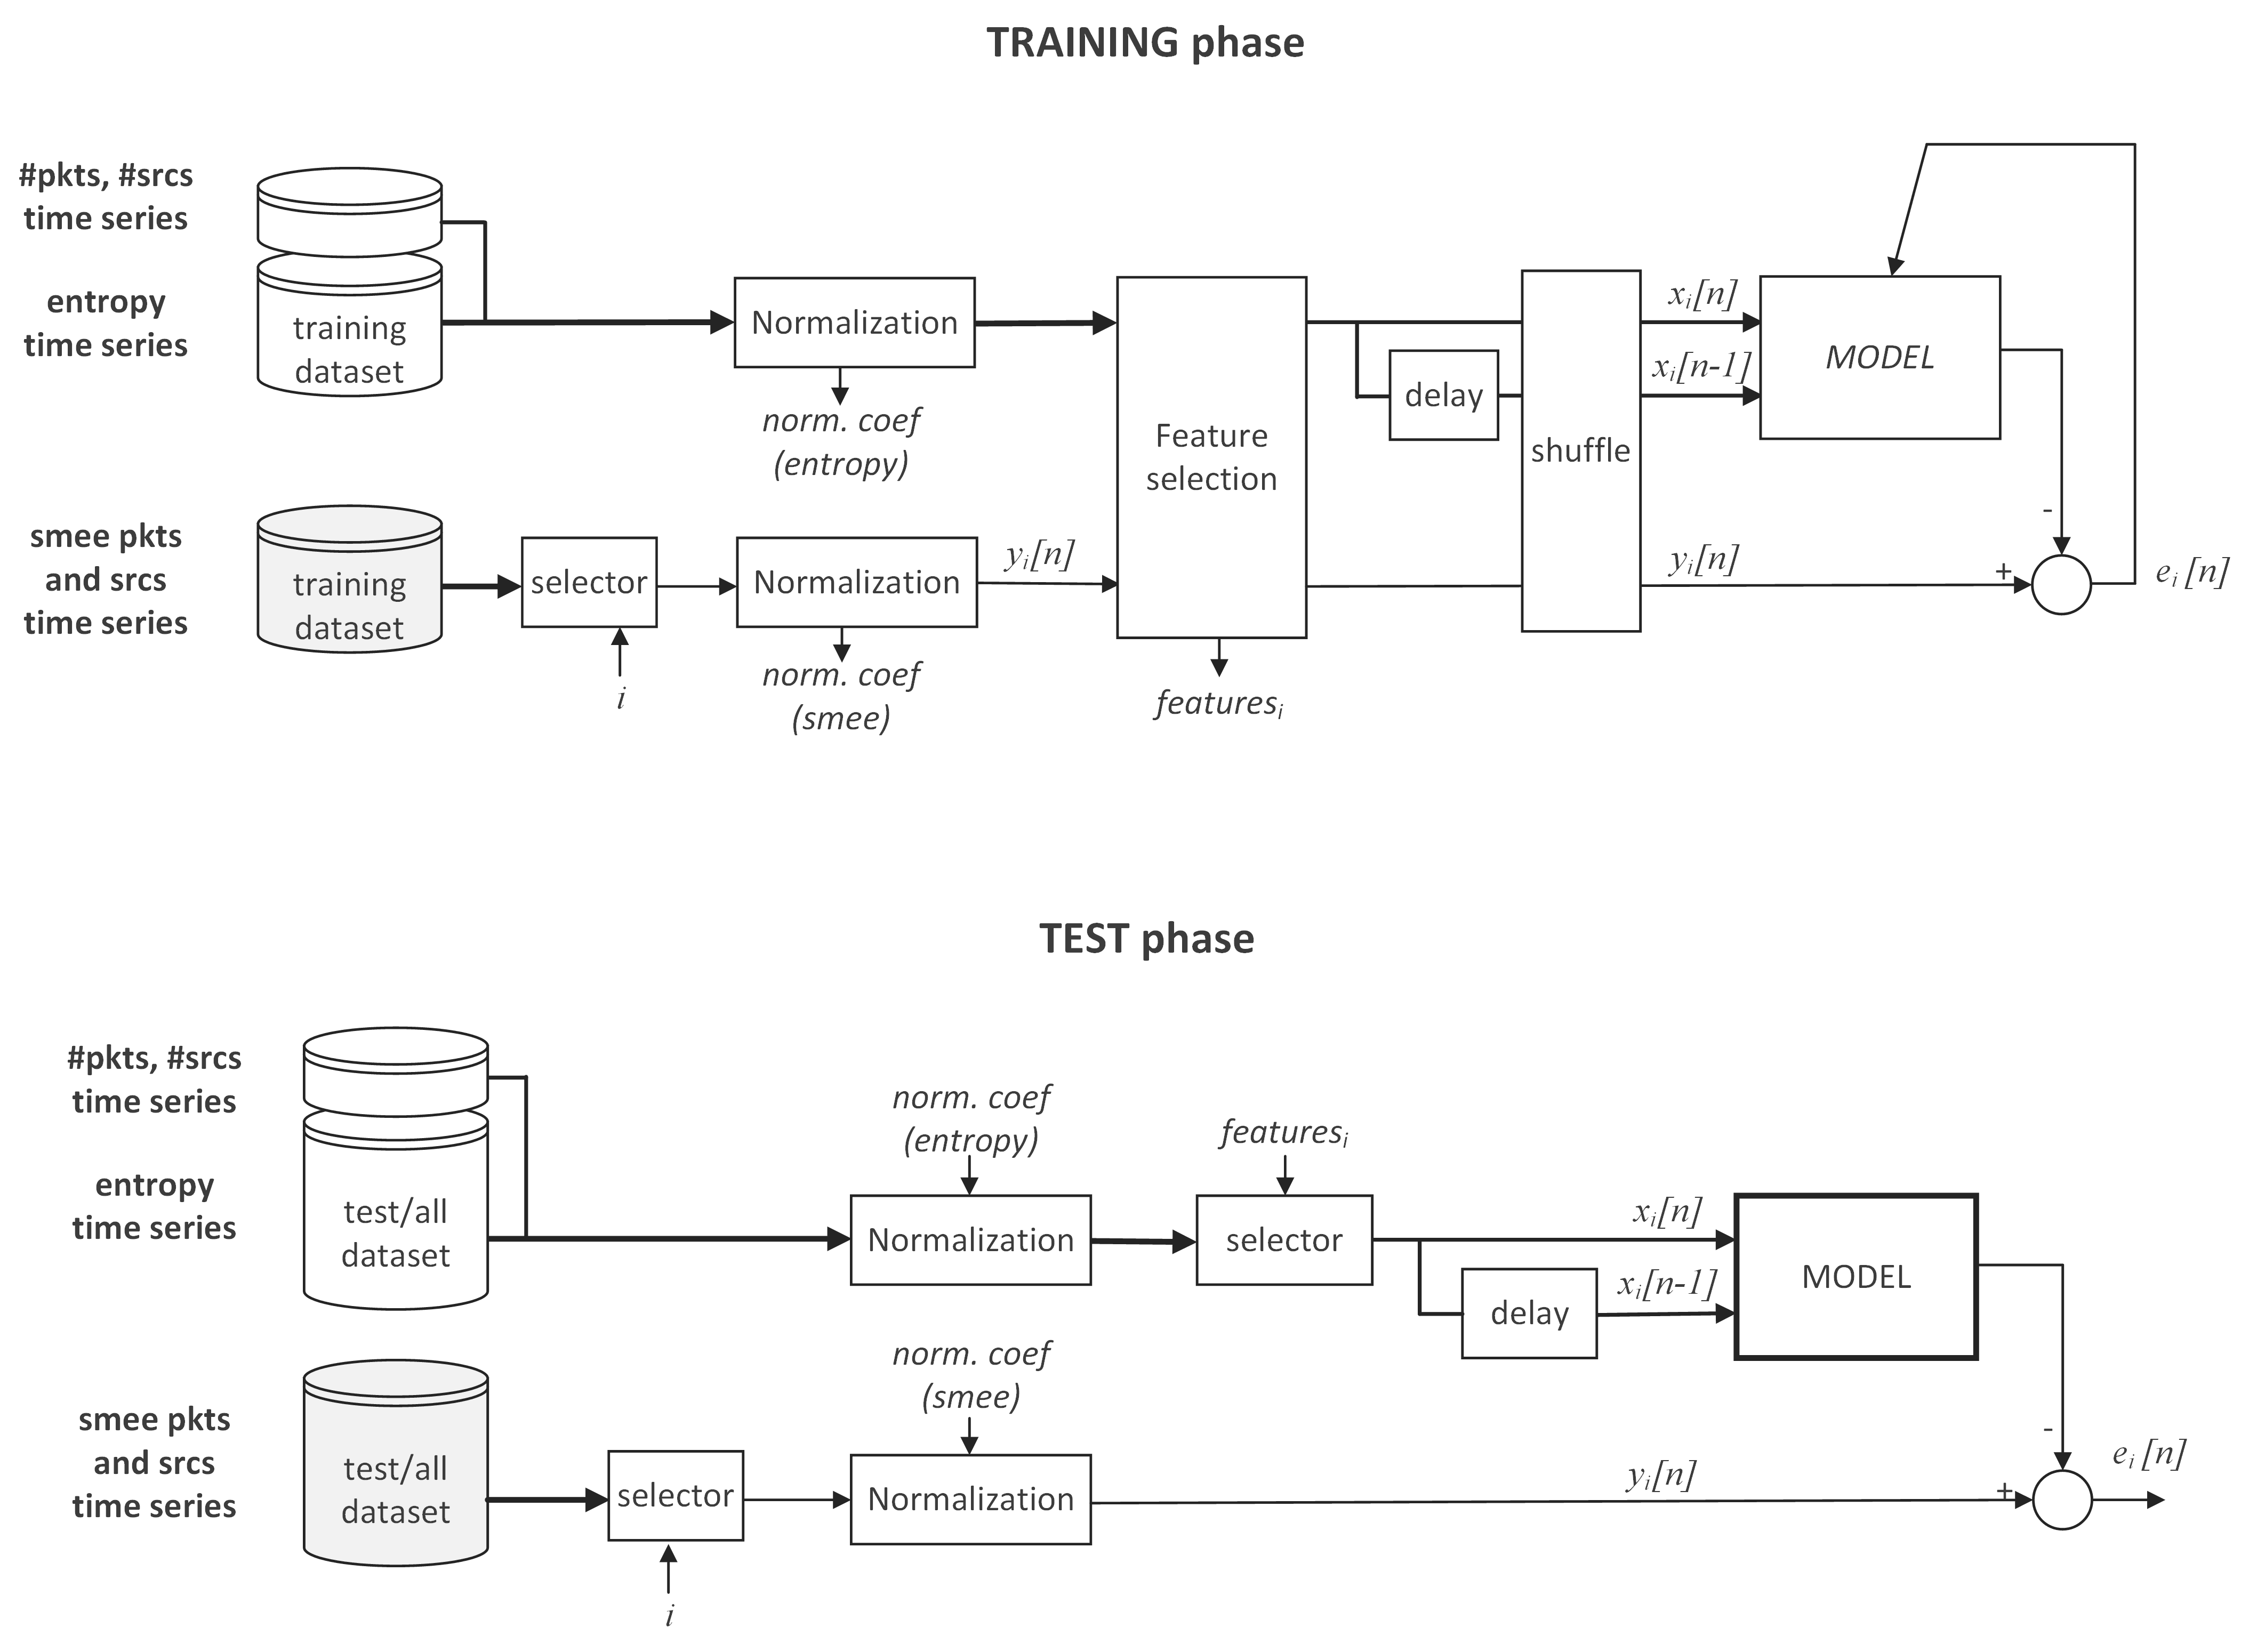
\includegraphics[width=0.95\linewidth]{graphics/modeling-example}
	\caption{Describe in the caption exactly what can be seen in the figure}
	\label{fig:modeling-example}
\end{figure}

\section{Subsets}

In hope of making any possible positive results more salient, we devised an extreme scenario where we limit the labeled date available for fine-tuning to a bare minimum of 10 records per attack category present in the original dataset. We then include an amount of benign records to keep the ratio of attack/benign flows of the original dataset. This results in the two subsets elaborated in tables \ref{table:methodology:datasets:cic17_subset} and \ref{table:methodology:datasets:unsw15_subset} labeled CIC17 and UNSW15 for the corresponding datasets.

\begin{table}[H]
	\centering
	\begin{tabular}{ccc}
		\thead{\textbf{\#}} & \thead{\textbf{Class}} & \thead{\textbf{No. Records}} \\ \hline \midrule
		0  & Botnet ARES             & 10  \\
		1  & FTP-Patator             & 10  \\
		2  & SSH-Patator             & 10  \\
		3  & DDoS LOIT               & 10  \\
		4  & DoS GoldenEye           & 10  \\
		5  & DoS Hulk                & 10  \\
		6  & DoS Slowhttptest        & 10  \\
		7  & DoS slowloris           & 10  \\
		8  & Heartbleed              & 10  \\
		9  & Infiltration            & 10  \\
		10 & Benign                  & 391 \\
		11 & PortScan - Firewall off & 10  \\
		12 & PortScan - Firewall on  & 10  \\
		13 & SQL Injection           & 10  \\
		14 & XSS WebAttack           & 10                    
	\end{tabular}
	\caption{Subset \textbf{CIC17} devised for CIC-IDS-2017 to include a minimal amount of records amounting to approximately 0.023\% of the total dataset.}
	\label{table:methodology:datasets:cic17_subset}
\end{table}

\begin{table}[H]
	\centering
	\begin{tabular}{ccc}
		\thead{\textbf{\#}} & \thead{\textbf{Class}} & \thead{\textbf{\textbf{No. Records}}} \\ \hline \midrule
		0 & Analysis       & 534     \\
		1 & Backdoors      & 397     \\
		2 & DoS            & 3972    \\
		3 & Exploits       & 29281   \\
		4 & Fuzzers        & 20848   \\
		5 & Generic        & 4301    \\
		6 & Benign         & 1991349 \\
		7 & Reconnaissance & 11971   \\
		8 & Shellcode      & 1546    \\
		9 & Worms          & 185                     
	\end{tabular}
	\caption{Subset \textbf{UNSW15} devised for UNSW-NB15 to include a minimal amount of records amounting to approximately 0.11\% of the total dataset.}
	\label{table:methodology:datasets:unsw15_subset}
\end{table}

\newpage